\documentclass[a4paper]{article}

\usepackage{pgfplots}

\pgfplotsset{compat=1.4}

\begin{document}

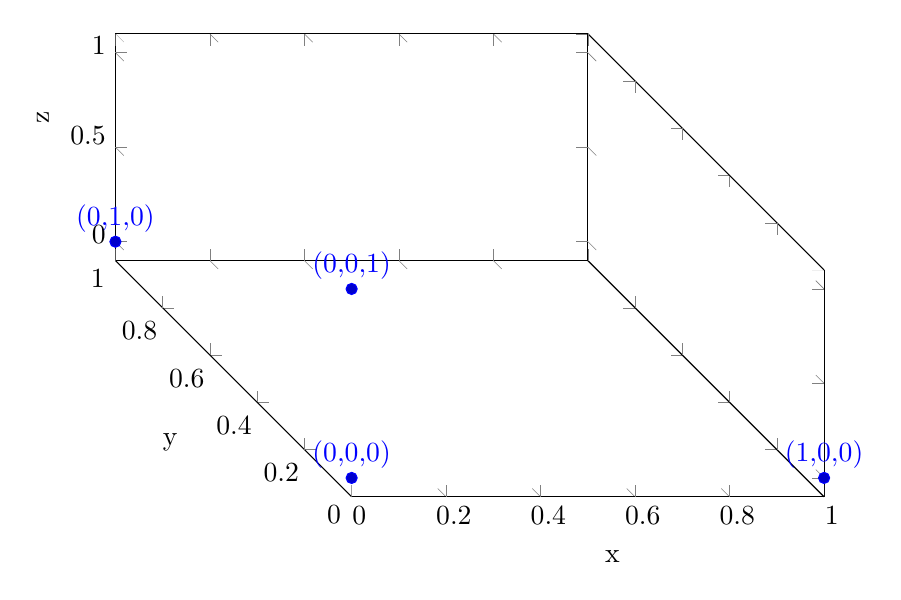
\begin{tikzpicture}
	\begin{axis}[
	%	scale mode=auto,% auto is default
		x={(6cm,0cm)},
		y={(-3cm,3cm)},
		z={(0cm,2.4cm)},
		xlabel=x,
		ylabel=y,
		zlabel=z,
	]

	\addplot3+[
		only marks,mark=*,
		nodes near coords,
		point meta={TeX code symbolic={
			\pgfmathprintnumberto[verbatim]{\pgfkeysvalueof{/data point/x}}\tempx
			\pgfmathprintnumberto[verbatim]{\pgfkeysvalueof{/data point/y}}\tempy
			\pgfmathprintnumberto[verbatim]{\pgfkeysvalueof{/data point/z}}\tempz
			\edef\pgfplotspointmeta{(\tempx,\tempy,\tempz)}}%
		}
	]
	coordinates {
		(0,0,0) (1,0,0) (0,1,0) (0,0,1)
	};
		
	\end{axis}
\end{tikzpicture}

\end{document}

